\documentclass[aspectratio=169]{beamer}

% MicroCD Labs technical capabilities deck.
% Compile with: pdflatex microcd_capabilities_deck.tex

\usepackage{graphicx}
\usepackage{tikz}

\usetheme{default}
\usefonttheme{professionalfonts}
\setbeamertemplate{navigation symbols}{}
\setbeamertemplate{footline}{%
  \hfill{\scriptsize\color{MicroCDMuted}\insertframenumber/\inserttotalframenumber}\hspace{1em}\vspace{0.6em}
}

\definecolor{MicroCDGreen}{HTML}{0F766E}
\definecolor{MicroCDDark}{HTML}{18211F}
\definecolor{MicroCDMuted}{HTML}{5D6965}
\definecolor{MicroCDSoft}{HTML}{F4F8F6}
\definecolor{MicroCDCoral}{HTML}{D85B45}
\definecolor{MicroCDAmber}{HTML}{D79A2B}

\setbeamercolor{normal text}{fg=MicroCDDark,bg=white}
\setbeamercolor{frametitle}{fg=MicroCDDark,bg=white}
\setbeamercolor{structure}{fg=MicroCDGreen}
\setbeamercolor{itemize item}{fg=MicroCDGreen}
\setbeamercolor{enumerate item}{fg=MicroCDGreen}

\setbeamerfont{frametitle}{size=\Large,series=\bfseries}
\setlength{\parindent}{0pt}
\setlength{\parskip}{0.45em}

\newcommand{\eyebrow}[1]{{\footnotesize\bfseries\color{MicroCDCoral}\MakeUppercase{#1}}\vspace{0.55em}}
\newcommand{\muted}[1]{{\color{MicroCDMuted}#1}}
\newcommand{\pill}[1]{%
  \tikz[baseline=(text.base)]{
    \node[
      fill=MicroCDSoft,
      draw=MicroCDGreen!20,
      rounded corners=4pt,
      inner xsep=8pt,
      inner ysep=5pt
    ] (text) {\small\bfseries #1};
  }%
}
\newcommand{\roaditem}[3]{%
  \begin{minipage}[t]{0.23\textwidth}
    {\large\bfseries\color{MicroCDGreen}#1}

    \vspace{0.4em}
    {\bfseries #2}

    \vspace{0.25em}
    {\footnotesize\color{MicroCDMuted}#3}
  \end{minipage}
}
\newcommand{\techcard}[3]{%
  \begin{minipage}[t]{0.31\textwidth}
    \colorbox{MicroCDSoft}{%
      \begin{minipage}[t][0.23\textheight][t]{0.92\linewidth}
        \vspace{0.75em}
        {\footnotesize\bfseries\color{MicroCDGreen}#1}

        \vspace{0.45em}
        {\bfseries #2}

        \vspace{0.3em}
        {\footnotesize\color{MicroCDMuted}#3}
      \end{minipage}
    }
  \end{minipage}
}

\begin{document}

\begin{frame}[plain]
  \begin{tikzpicture}[remember picture,overlay]
    \node[anchor=center] at (current page.center) {%
      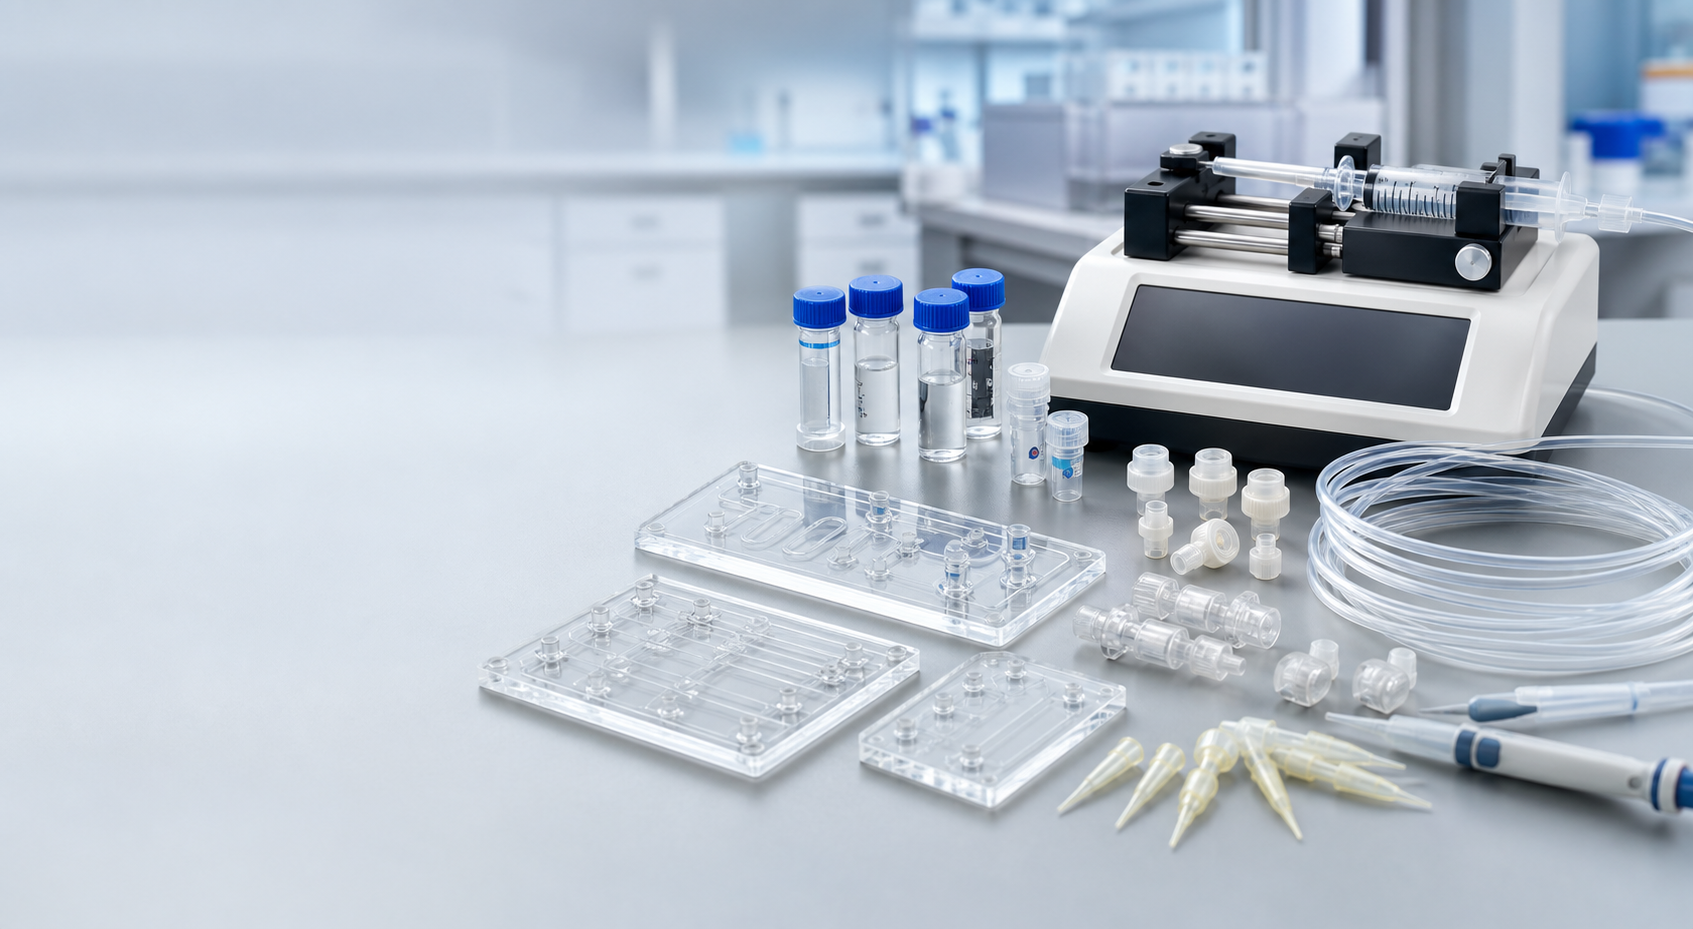
\includegraphics[width=\paperwidth,height=\paperheight]{assets/hero-lab-supply.png}
    };
    \fill[MicroCDDark,opacity=0.76] (current page.south west) rectangle ([xshift=0.62\paperwidth]current page.north west);
    \fill[MicroCDDark,opacity=0.18] ([xshift=0.62\paperwidth]current page.south west) rectangle (current page.north east);
  \end{tikzpicture}

  \vspace{2.1em}
  {\footnotesize\bfseries\color{MicroCDCoral}TECHNICAL CAPABILITIES}

  \vspace{1.1em}
  {\Huge\bfseries\color{white} MicroCD Labs}

  \vspace{0.45em}
  {\Large\color{white} Microfluidics, assay development, LFIA workflows, and diagnostic product translation.}

  \vfill
  {\footnotesize\color{white} Snehan Peshin, Ph.D. \quad | \quad info@microcdlabs.com}
\end{frame}

\begin{frame}{Ph.D. background}
  \eyebrow{Scientific and product background}

  \begin{columns}[T]
    \begin{column}{0.52\textwidth}
      {\Large\bfseries Snehan Peshin, Ph.D.}

      \vspace{0.7em}
      \muted{Biomedical R\&D experience spanning diagnostics, assay development, lab-on-a-disc systems, microfluidics, and applied product development.}

      \vspace{1em}
      \pill{Ph.D., UC Irvine}\quad
      \pill{Zoetis}

      \vspace{0.6em}
      \pill{BlueJay Diagnostics}\quad
      \pill{Vanderbilt}
    \end{column}
    \begin{column}{0.40\textwidth}
      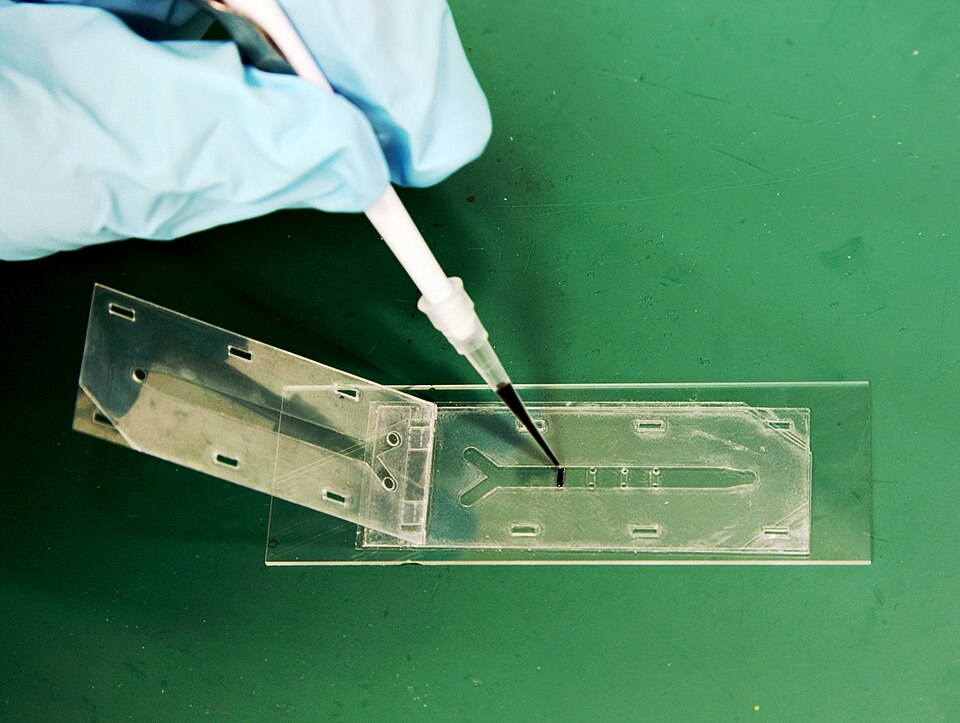
\includegraphics[width=\linewidth,height=0.52\textheight]{assets/deck-images/microfluidic-device.jpg}
    \end{column}
  \end{columns}
\end{frame}

\begin{frame}{Technical expertise}
  \eyebrow{What engineers will care about}

  \begin{columns}[T]
    \begin{column}{0.48\textwidth}
      \begin{itemize}
        \item Diagnostic workflow architecture
        \item Lab-on-a-disc fluid handling
        \item LFIA workflow experience
        \item Assay-to-cartridge translation
      \end{itemize}
    \end{column}
    \begin{column}{0.48\textwidth}
      \begin{itemize}
        \item Microfluidic layout and routing
        \item Rapid prototype iteration
        \item Consumable and cartridge design inputs
        \item System integration and test planning
      \end{itemize}
    \end{column}
  \end{columns}

  \vspace{1.1em}
  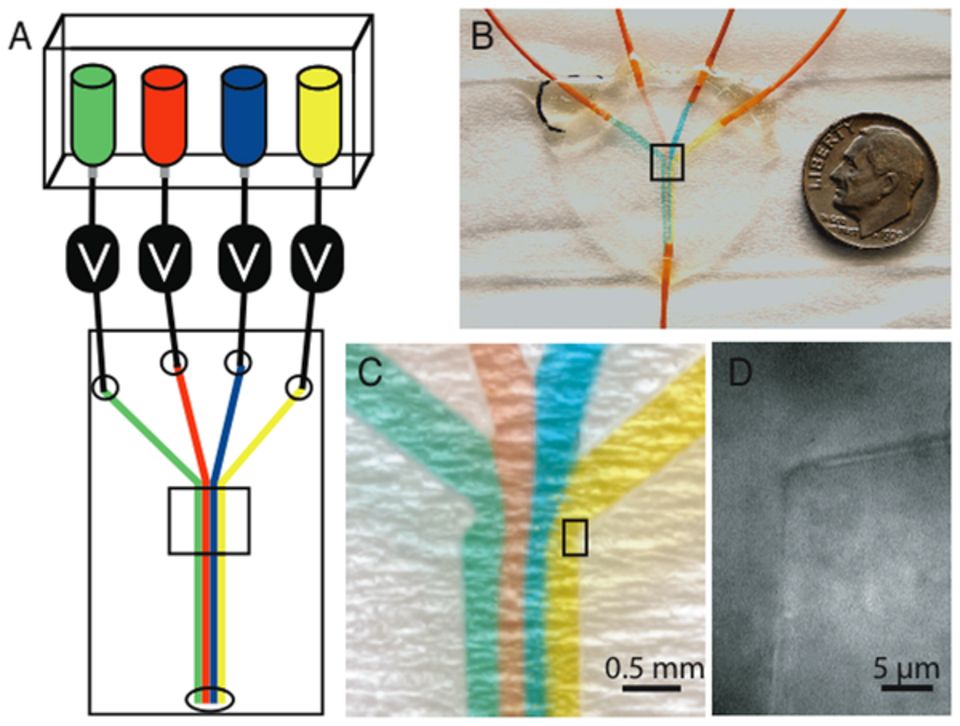
\includegraphics[width=\linewidth,height=0.28\textheight]{assets/deck-images/laminar-flow.png}
\end{frame}

\begin{frame}{Diagnostics expertise}
  \eyebrow{Workflow-first development}

  \begin{columns}[T]
    \begin{column}{0.52\textwidth}
      {\large\bfseries Diagnostic systems are more than a chip.}

      \vspace{0.6em}
      \muted{MicroCD Labs approaches diagnostics as an integrated workflow: sample handling, reagent timing, assay readout, consumable constraints, and user steps.}

      \vspace{0.8em}
      \begin{itemize}
        \item Sample-to-answer workflow thinking
        \item Point-of-care and low-resource constraints
        \item Assay robustness and usability tradeoffs
        \item Early technical risk identification
      \end{itemize}
    \end{column}
    \begin{column}{0.40\textwidth}
      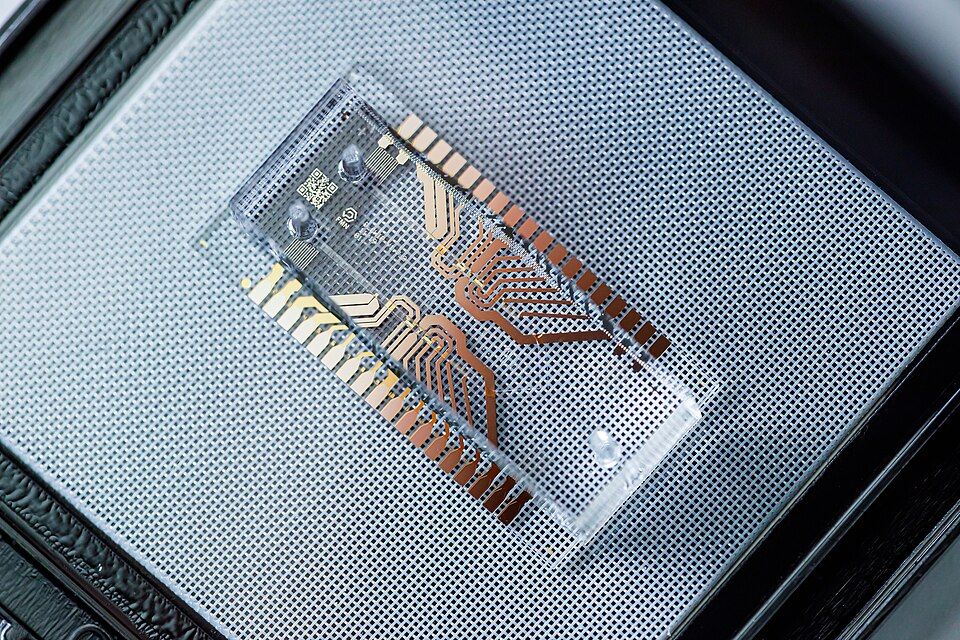
\includegraphics[width=\linewidth,height=0.52\textheight]{assets/deck-images/chip.jpg}
    \end{column}
  \end{columns}
\end{frame}

\begin{frame}{Assay development capabilities}
  \eyebrow{Bench chemistry to device workflow}

  \techcard{01}{Assay feasibility}{Protocol review, reagent constraints, sample inputs, timing, and early readout decisions.}
  \hfill
  \techcard{02}{LFIA experience}{Lateral-flow style assay thinking, strip workflow constraints, conjugate/reagent handling, and readout needs.}
  \hfill
  \techcard{03}{Microfluidic translation}{Converting assay steps into flow paths, incubation zones, metering concepts, and cartridge requirements.}

  \vspace{1.1em}
  \muted{The goal is to identify what must be true biologically and physically before locking into a consumable or instrument design.}
\end{frame}

\begin{frame}{Lab-on-a-disc work}
  \eyebrow{Centrifugal microfluidic thinking}

  \begin{columns}[T]
    \begin{column}{0.48\textwidth}
      \begin{itemize}
        \item Disc-based fluid routing concepts
        \item Passive timing and delayed-flow ideas
        \item Chamber, channel, and venting considerations
        \item Assay workflow mapping onto rotational formats
      \end{itemize}
    \end{column}
    \begin{column}{0.46\textwidth}
      \colorbox{MicroCDSoft}{%
        \begin{minipage}[c][0.46\textheight][c]{0.92\linewidth}
          \centering
          {\Large\bfseries Lab-on-disc focus}

          \vspace{0.8em}
          \muted{Useful where workflow simplification, contained consumables, and low-complexity operation matter.}
        \end{minipage}
      }
    \end{column}
  \end{columns}
\end{frame}

\begin{frame}{Fluidics design experience}
  \eyebrow{Design inputs before fabrication}

  \begin{columns}[T]
    \begin{column}{0.50\textwidth}
      \begin{itemize}
        \item Channel and chamber layout planning
        \item Connector, tubing, and pump interface choices
        \item Flow path simplification
        \item Material and manufacturability constraints
        \item Prototype test fixtures and benchtop validation
      \end{itemize}
    \end{column}
    \begin{column}{0.42\textwidth}
      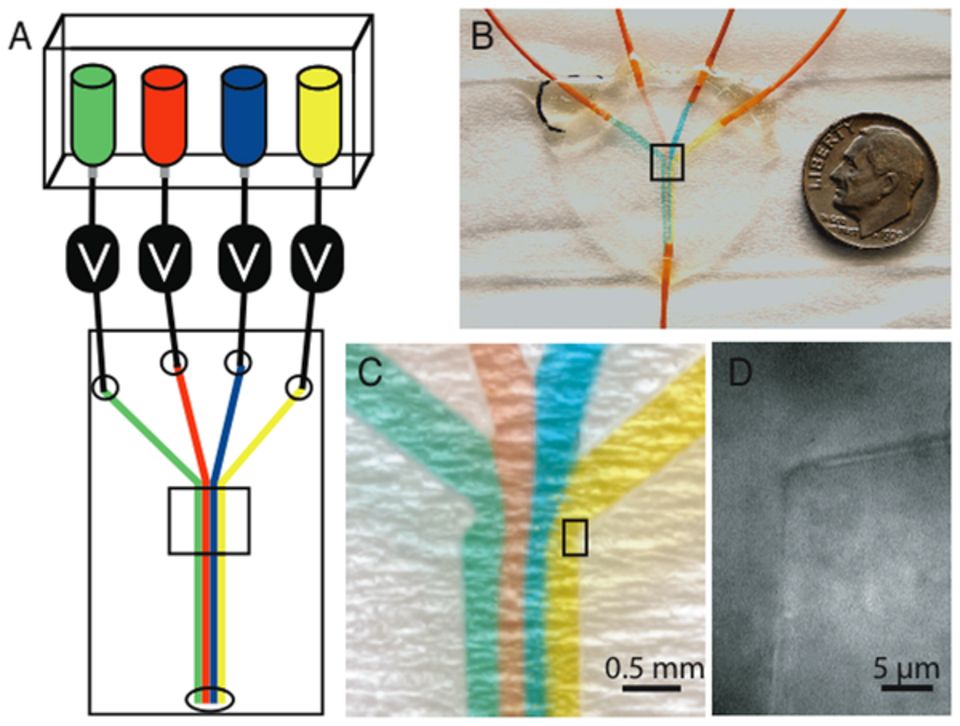
\includegraphics[width=\linewidth,height=0.48\textheight]{assets/deck-images/laminar-flow.png}
    \end{column}
  \end{columns}
\end{frame}

\begin{frame}{Product development experience}
  \eyebrow{From technical concept to usable product}

  \begin{columns}[T]
    \begin{column}{0.48\textwidth}
      {\large\bfseries Development activities}

      \begin{itemize}
        \item Requirements definition
        \item Prototype planning
        \item Design iteration
        \item Test method thinking
        \item Supplier and fabrication coordination
      \end{itemize}
    \end{column}
    \begin{column}{0.45\textwidth}
      {\large\bfseries Product lens}

      \begin{itemize}
        \item Usability and workflow fit
        \item Cost and manufacturability awareness
        \item Consumable repeatability
        \item Partner/OEM integration paths
      \end{itemize}
    \end{column}
  \end{columns}
\end{frame}

\begin{frame}{Example projects}
  \eyebrow{Representative project types}

  \techcard{A}{Lab-on-disc assay workflow}{Map sample, reagent, timing, and readout steps into a centrifugal microfluidic format.}
  \hfill
  \techcard{B}{LFIA-to-cartridge concept}{Translate lateral-flow assay constraints into a more controlled consumable or workflow.}
  \hfill
  \techcard{C}{Microfluidic prototype kit}{Define chip, holder, tubing, fitting, pump, and test setup for early assay feasibility.}

  \vspace{1em}
  \techcard{D}{OEM consumable exploration}{Develop early requirements for custom cartridges or partner-specific research consumables.}
  \hfill
  \techcard{E}{Diagnostic workflow review}{Identify technical risks before committing to fabrication or instrument design.}
  \hfill
  \techcard{F}{Fluidics troubleshooting}{Review flow path, bubbles, dead volume, interfaces, and test setup issues.}
\end{frame}

\begin{frame}{Future product roadmap}
  \eyebrow{Near-term supply, long-term product platform}

  \roaditem{01}{Research tools}{Starter kits, chips, fittings, pumps, and useful lab accessories.}
  \hfill
  \roaditem{02}{OEM cartridges}{Custom consumables for partner assays and instrument workflows.}
  \hfill
  \roaditem{03}{Point-of-care diagnostics}{Lab-on-disc and cartridge-based workflows for accessible testing.}
  \hfill
  \roaditem{04}{Custom consumables}{Application-specific parts for pilot studies and repeat research use.}

  \vspace{1.5em}
  \muted{The roadmap starts practical: support researchers today while building toward higher-value diagnostic and consumable products.}
\end{frame}

\begin{frame}{Partnership opportunities}
  \eyebrow{Where collaboration may help}

  \begin{columns}[T]
    \begin{column}{0.48\textwidth}
      {\large\bfseries Technical partnership areas}

      \begin{itemize}
        \item Prototype fabrication
        \item Glass and polymer microfluidics partners
        \item Design for manufacturing
        \item Pilot production
        \item Assay and OEM cartridge partners
        \item Point-of-care diagnostic collaborators
      \end{itemize}
    \end{column}
    \begin{column}{0.44\textwidth}
      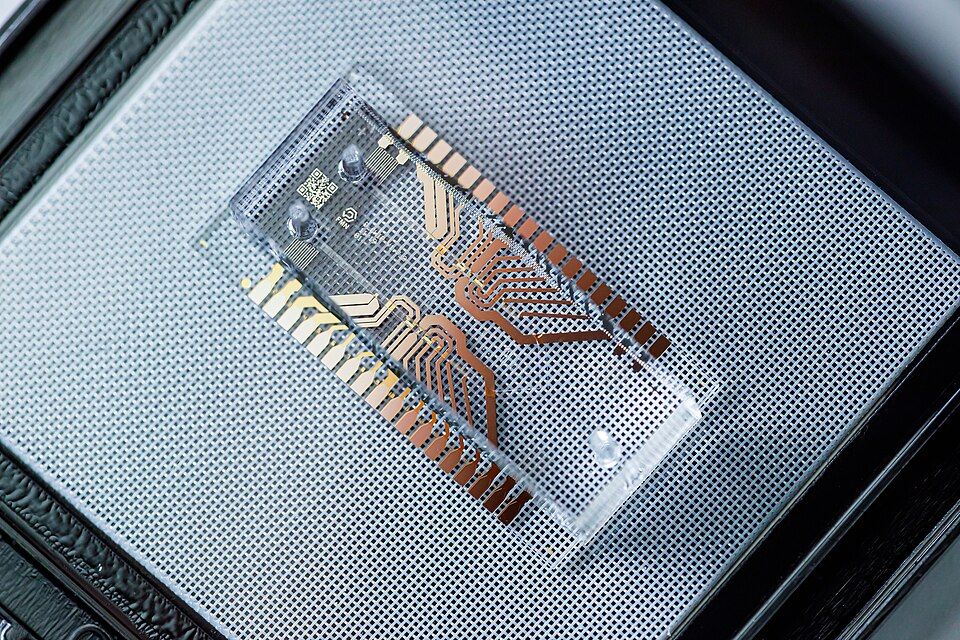
\includegraphics[width=\linewidth,height=0.48\textheight]{assets/deck-images/chip.jpg}
    \end{column}
  \end{columns}

  \vspace{0.8em}
  {\footnotesize\color{MicroCDMuted}Potential partners may include microfluidic fabricators, assay developers, diagnostic companies, academic labs, and OEM instrument teams.}
\end{frame}

\begin{frame}{Future commercial products}
  \eyebrow{Product directions}

  \begin{columns}[T]
    \begin{column}{0.31\textwidth}
      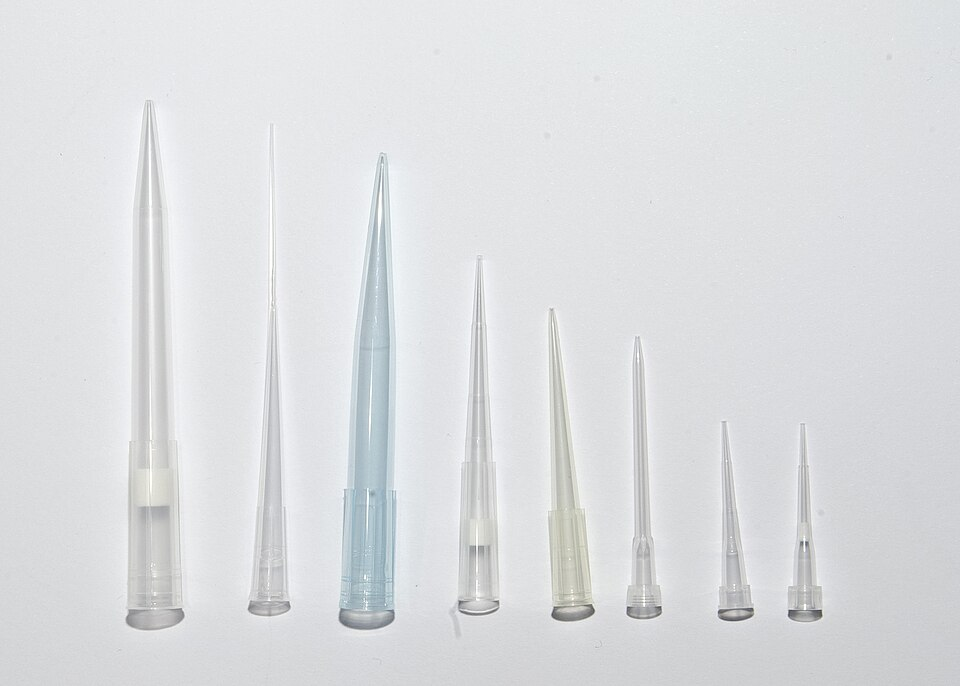
\includegraphics[width=\linewidth,height=0.23\textheight]{assets/deck-images/pipette-tips.jpg}

      \vspace{0.55em}
      {\bfseries Research-use supply kits}

      {\footnotesize\color{MicroCDMuted}Bundled parts for fast setup and repeat purchasing.}
    \end{column}
    \begin{column}{0.31\textwidth}
      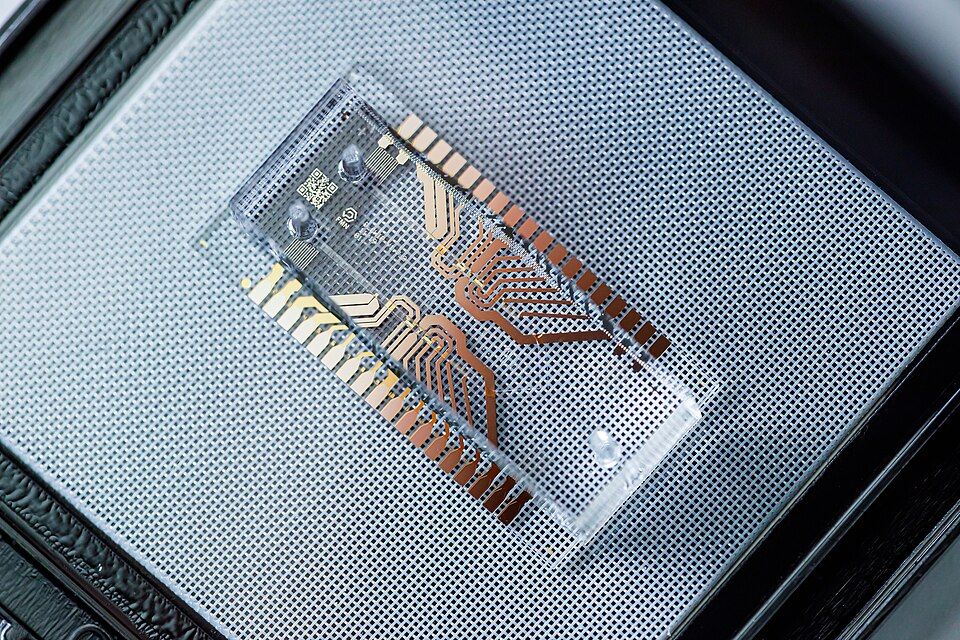
\includegraphics[width=\linewidth,height=0.23\textheight]{assets/deck-images/chip.jpg}

      \vspace{0.55em}
      {\bfseries Custom cartridges}

      {\footnotesize\color{MicroCDMuted}Application-specific consumables for assay partners.}
    \end{column}
    \begin{column}{0.31\textwidth}
      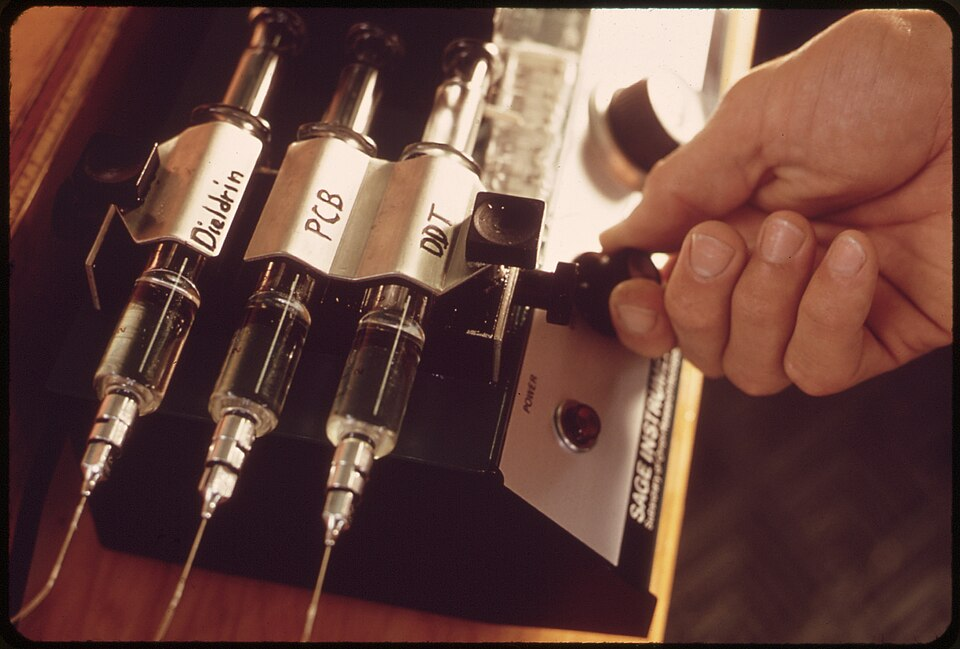
\includegraphics[width=\linewidth,height=0.23\textheight]{assets/deck-images/syringe-pump.jpg}

      \vspace{0.55em}
      {\bfseries Integrated test workflows}

      {\footnotesize\color{MicroCDMuted}Benchtop and point-of-care systems for future diagnostic use cases.}
    \end{column}
  \end{columns}

  \vspace{1em}
  \muted{Next step: discuss a target use case, prototype path, and early customer need.}
\end{frame}

\begin{frame}[plain]
  \begin{tikzpicture}[remember picture,overlay]
    \fill[MicroCDSoft] (current page.south west) rectangle (current page.north east);
    \fill[MicroCDGreen] (current page.south west) rectangle (0.12\paperwidth,\paperheight);
  \end{tikzpicture}

  \hspace{0.9cm}
  \begin{minipage}{0.78\textwidth}
    \vspace{2.4em}
    {\footnotesize\bfseries\color{MicroCDCoral}CONTACT}

    \vspace{1.1em}
    {\Huge\bfseries MicroCD Labs}

    \vspace{0.6em}
    {\Large Microfluidics, diagnostic innovation, and research-use supply.}

    \vspace{1.3em}
    Email: \texttt{info@microcdlabs.com}

    Website: \texttt{sites.google.com/view/microcd-labs/home}
  \end{minipage}
\end{frame}

\end{document}
